\chapter{Graphical and numerical diagnostic tools to assess multiple imputation models by posterior predictive checking}
\chaptermark{Diagnostics for imputation models}
\label{chap6}
	\begin{abstract}
		We propose a method to diagnose imputation models based on posterior predictive checking. To assess the congeniality of imputation models, we compare the observed data with their replicates generated under corresponding posterior predictive distributions. The idea is that if the imputation model is congenial with the substantive model, the observed data is expected to locate in the centre of corresponding predictive posterior distributions. We investigate the proposed diagnostic method for parametric and non-parametric imputation approaches, continuous and discrete incomplete variables, univariate and multivariate missingness patterns. The results show the validity of the proposed diagnostic method.  	
	\end{abstract}
	
	\section{Introduction}
	\label{sec:6.1}
	Multiple imputation (MI) is a popular approach for the analysis of incomplete datasets. It involves generating several plausible imputed datasets and aggregating different results into a single inference. Missing cells are filled with synthetic data drawn from corresponding posterior predictive distributions. This procedure is repeated multiple times, resulting in several imputed datasets. The parameters of scientific interest are then estimated for each imputed dataset by complete-data analyses. Finally, different estimates are pooled into one inference using Rubin's rule, which accounts for within and across imputation uncertainty \citep{RubinD1987}. 
	
	A crucial part of the multiple imputation process is selecting sensible models to generate plausible values for the missing data. The validity of post-imputation analyses relies on the congeniality of the imputation model and the substantive model of interest \citep{meng1994multiple}. However, model selection is not a trivial process in practice since there can be a wide array of candidate models to check. Therefore, researchers should consider which variables, interaction terms, and nonlinear terms are included based on the scientific interest and data features.  
	
	Despite the popularity of multiple imputation, there are only a few imputation model diagnostic methodologies. One standard diagnostic method is to compare distributions of the observed with imputed data \citep{Buuren2018, abayomi2008diagnostics}. Plausible imputation models would generate imputed values that have a similar distribution to the observed data. Although missing at random (MAR) mechanisms would also induce the discrepancies between the observed and imputed data, any dramatic departures that the observed data features cannot explain are evidence of potential imputation model misspecification. Reliable interpretation of the observed and imputed data's discrepancies could be derived from external knowledge about the incomplete variables and the missingness mechanisms \citep{abayomi2008diagnostics}. 
	
	The idea to evaluate the validity of scientific models with multiply imputed data is not new. \citet{bondarenko2016graphical} proposed an advanced diagnostic method to compare the distributions of the observed with imputed data conditional on the probability of missingness. \citet{gelman1998not} applied cross-validation to check the fit of a hierarchical Bayesian model in the study of 51 public opinion polls preceding the 1988 U.S. Presidential election. \citet{gelman2005multiple} also proposed to apply graphical posterior predictive inference on the test statistics for model checking with missing and latent data. If regression-based imputation approaches are involved, the conventional regression diagnostics, such as plots of residuals and outliers, are helpful \citep{white2011multiple}. A comprehensive overview of model diagnostic in multiple imputation is available in \citet{nguyen2017model}.
	
	Posterior predictive checking (PPC) has been proposed as an alternative method for the imputation model diagnostic \citep{gelman2005multiple, he2012diagnosing, nguyen2015posterior}. PPC is a Bayesian model checking approach that compares the replicated data drawn from the corresponding posterior predictive distribution to the observed data. If the model lacks fit, there could be a discrepancy between the replicated and observed data. 
	
	\citet{he2012diagnosing} and \citet{nguyen2015posterior} applied posterior predictive checking to assess the inadequacies of the joint imputation model with one or more test quantities relative to the scientific interest. To evaluate the `usability' of imputation models with respect to the test statistics, analysts compare the estimates for the complete data to their replicates. Comparisons of the complete data and its replicates ensure the calculation of test quantities with general missingness patterns. However, it also results in sensitivity to the amount of missingness.    
	
	This manuscript proposes and evaluates the implementation of posterior predictive checking for imputation techniques. The general idea is that if the imputation model is congenial to the substantive model, the expected value of the data (whether observed or missing) is in the centre of corresponding predictive posterior distributions. We compare the observed data to their posterior replicates generated under the imputation model and evaluate the posterior distributions of all observed data points. This distinguishes our approach from the posterior predictive checking of imputation models by applying target analyses. We demonstrate:
	\begin{enumerate}
		\item that PPC can be generalised to variable-by-variable imputation techniques; 
		\item that PPC can be used to identify the imputation model that conforms most to the true data generating model;
		\item that PPC can be used as a model evaluation technique to identify the better substantive analysis model;
		\item how to perform PPC with \texttt{MICE} in \texttt{R} on a real-life data set \citep{Buuren2011};
		\item that this PPC approach is not sensitive to the amount of missing data.
	\end{enumerate}
	The remainder of this manuscript is organised as follows. In section \ref{sec:6.2}, we review the posterior predictive checking of the imputation model by applying the target analysis proposed by \citet{he2012diagnosing}. In section \ref{sec:6.3}, we provide an overview of the \texttt{MICE} package and the underlying imputation algorithm: fully conditional specification (FCS). We also further point out the necessity of extending the posterior predictive checking of the imputation model so that the diagnostics would apply to the \texttt{MICE} algorithm. In section \ref{sec:6.4}, we evaluate the performance of the proposed diagnostic approach with simulation studies. In section \ref{sec:6.5}, we show the results of simulation studies. In section \ref{sec:6.6}, we apply the proposed diagnostic approach to the body mass index (BMI) data in Dutch. In section \ref{sec:6.7}, we conclude with a discussion of our findings.  
	
	\section{Posterior predictive checking (PPC)}
	\label{sec:6.2}
	\subsection{Posterior predictive checking}
	Without incomplete variables, PPC compares the observed data $y$ with the replicated data $y^{rep}$ which are simulated from the posterior predictive distribution, with parameter $\theta$:
	\begin{equation}
		\begin{array}{ll}
			p(y^{rep}|y) = \int p(y^{rep}|\theta)p(\theta|y)d\theta
		\end{array} 
	\end{equation}
	To detect the discrepancy between the model and the data, we define test quantities that reflect the scientific interest and estimate them for both observed and replicated data. Misfits of the model with respect to the data could be summarised by the posterior predictive p-value, which is the probability that the replicated data are more extreme than the observed data, with respect to the selected test quantities \citep{gelman2013bayesian}:
	\begin{equation}
		\begin{array}{ll}
			p_{B} &= Pr(T(y^{rep}, \theta) \ge T(y, \theta)|y)\\
			&= \int\int I_{T(y^{rep}, \theta) \ge T(y, \theta)}p(y^{rep}|\theta)p(\theta|y)dy^{rep}d\theta,
		\end{array} 
	\end{equation}
	where $I$ is the indicator function. An extreme p-value (close to 0 or 1) implies the suspicion on the fit of the model since a consistent discrepancy between test quantities $T(y^{rep}, \theta)$ and $T(y, \theta)$ cannot be explained by the simulation variance. 
	
	Posterior predictive checking has been widely used for model diagnostic in applied Bayesian analysis \citep[chapter 6]{gelman2013bayesian}, and the posterior predictive distribution is usually calculated by simulation. Suppose we have $N$ draws of model parameters from its posterior distribution $\theta_j, j=1,\dots,N$, we then generate a replicated data for every theta $\theta_j$. The PPC compares test quantities based on observed data with the empirical predictive distribution of test quantities. The estimated posterior predictive p-value is the proportion of these \texttt{N} simulations for which $T_{j}(y^{rep}, \theta) > T_{j}(y, \theta)$. It is noticeable that PPC's application for the imputation model diagnostic is not based on the hypothesis test perspective. Hence, there is no underlying assumed distribution for the posterior predictive p-value in this case. The posterior predictive p-value indicates whether the model would provide plausible inference based on the data with respect to the selected test quantities. 
	
	To perform multiple imputation model checking with PPC, we compare the completed data, the combination of the observed and imputed data, with its replications. \citet{gelman2005multiple} applied graphical PPC to visualise test quantities comparisons based on completed and replicated data. \citet{he2012diagnosing} and \citet{nguyen2015posterior} developed numerical posterior predictive checks as target analyses to the joint imputation model. \citet{he2012diagnosing} proposed two kinds of discrepancies, completed data discrepancy and expected completed-data discrepancy, and the approaches to calculate corresponding posterior predictive p-values. We briefly introduce these discrepancies and p-values for the completeness of PPC for MI models.
	
	\subsection{Completed-data discrepancy}
	To assess the completed-data discrepancy $T(y_{com}^{rep}, \theta) - T(y_{com}, \theta)$, we draw imputed values for incomplete variables $y_{mis}$ and the replication of the complete data $y_{com}^{rep}$ from their posterior predictive distribution:
	\begin{equation}
		\begin{array}{ll}
			p(y_{com}^{rep}, y_{mis}|y_{obs}) = \int p(y_{com}^{rep}|\theta)p(y_{mis}|y_{obs}, \theta)p(\theta|y_{obs})d\theta,
		\end{array} 
	\end{equation}
	where $y_{obs}$ is the observed data and $y_{com} = (y_{obs}, y_{mis})$. To assess the model fit, we calculate the posterior predictive p-value as :
	\begin{equation}
		\begin{array}{ll}
			p_{B, com} &= Pr(T(y_{com}^{rep}) \ge T(y_{com})|y_{obs})\\
			&= \int\int I_{T(y_{com}^{rep}) \ge T(y_{com})}p(y_{com}^{rep}, y_{mis}|y_{obs})dy_{com}^{rep}dy_{mis}
		\end{array} 
	\end{equation}
	The simulation process to estimate p-value proposed by \citet{he2012diagnosing} is:
	\begin{enumerate}
		\item Simulate $N$ draws of $\theta$ from the corresponding posterior distribution $p(\theta|y_{obs})$
		\item For each $\theta_{j}, j=1, \dots, N$, impute $y_{mis}^j$ from $p(y_{mis}|y_{obs}, \theta_{j})$ and simulate the replicated data $y_{com}^{rep, j}$ from $p(y_{com}^{rep}|\theta_{j})$
	\end{enumerate}
	A $p_{B, com}$, which is close to 0 or 1, implies the discrepancy between the model and the data with respect to the selected test quantities.  
	\subsection{Expected completed-data discrepancy}
	\citet{he2012diagnosing} noticed that the power of completed-data discrepancy is weakened because the variance of imputed data across complete data $y_{imp}$ and replicated data $y_{imp}^{rep}$ increase the variance of the test quantities. \citet{he2012diagnosing} reduced the variance of completed-data discrepancy by calculating the expectation value of missing data for each model parameter draw. 
	The modification of p-value $p_{B, ecom}$ would be:  
	\begin{equation}
		\begin{array}{ll}
			p_{B, ecom} &= Pr(E[T(y_{com}^{rep})|y_{obs}^{rep}, y_{obs}] \ge E[T(y_{com})|y_{obs}^{rep}, y_{obs}]|y_{obs})\\
			&= \int\int I_{E[T(y_{com}^{rep})|y_{obs}^{rep}, y_{obs}] \ge E[T(y_{com})|y_{obs}^{rep}, y_{obs}]}p(y_{obs}^{rep}, y_{obs})dy_{obs}^{rep}
		\end{array} 
	\end{equation}
	Again, the nested simulation process to calculate the p-value $p_{B, ecom}$ is:
	\begin{enumerate}
		\item Simulate $N_{1}$ draws of $\theta$ from the corresponding posterior distribution $p(\theta|y_{obs})$
		\item For each $\theta_{j}, j=1, \dots, N_{1}$, impute $y_{mis}^j$ from $p(y_{mis}|y_{obs}, \theta_{j})$ and simulate the replicated data $y_{com}^{rep, j}$ from $p(y_{com}^{rep}|\theta_{j})$
		\item For each j-th replicate, calculate the mean discrepancy by setting $y_{mis}^j$ and $y_{com}^{rep, j}$ to missing and overimputing them with the same paramters $\theta_{j}$ over $N_{2}$ draws $y_{mis}^{j, k}$ and $y_{com}^{rep, j, k}, k = 1, \dots, N_{2}$. Calculate the difference : $D_{j, k} = T(y_{obs}^{rep, j}, y_{mis}^{rep, j, k}) - T(y_{obs}, y_{mis}^{rep, j, k})$ over $N_{2}$ draws and then average the difference for the j-th replicate : $\bar{D}_{j.} = \sum_{1}^{k}D_{j, k}/k$
		\item Calculate $p_{B, ecom}$ as the proportion of these $N_{1}$ estimates that are positive, $\bar{D}_{j.} \ge 0$    
	\end{enumerate}
	
	\citet{he2012diagnosing} evaluated whether the PPC could detect the uncongeniality of the imputation model. \citet{nguyen2015posterior} investigated the performance of PPC in other imputation model misspecification scenarios, such as ignoring the response variable and auxiliary variables or failing to transform skewed variables. The PPC approach proposed by \citet{he2012diagnosing} is based on the joint imputation model. The imputation model for diagnostic is a joint distribution for the observed data, and the test quantities depend on multiple variables and parameters. 
	
	\section{\texttt{MICE} package}
	\label{sec:6.3}
	Fully conditional specification (FCS) is a popular approach for multiple imputation. It attempts to specify an imputation model for each missing variable $Y_j, j = 1, \dots, p$ conditional on all the other variables $P(Y_j | Y_{-j}, \theta_{j})$, with parameter $\theta_{j}$. It generates imputations iteratively over all missing variables after an initial imputation, such as mean imputation or random draw from observed values. Let $Y_{j}^{t} = (Y_{j}^{obs}, Y_{j}^{mis(t)})$ denote the observed and imputed values of variable $Y_{j}$ at iteration $t$ and $Y_{-j}^{t} = (Y_{1}^{t}, \dots, Y_{j-1}^{t}, Y_{j+1}^{t-1}, \dots, Y_{p}^{t-1})$. Given the most recent imputations of the other missing variables $Y_{j}^{t}$ at iteration $t$, the algorithm of generating imputations for the missing variable $Y_{j}$ consists of the following draws:
	\begin{align*}
		\theta_{j}^{t} \sim f(\theta_{j})f(Y_{j}^{obs}|Y_{-j}^{t}, \theta_{j})\\
		Y_{j}^{mis(t)} \sim f(Y_{j}^{mis}|Y_{-j}^{t}, \theta_{j}^{t}),
	\end{align*}
	where $f(\theta_{j})$ is the prior distribution for the parameter of the imputation model $\theta_{j}$.
	The FCS is an attractive imputation approach because of its flexibility in imputation model specification. It is known under different names: chained equations stochastic relaxation, variable-by-variable imputation, switching regression, sequential regressions, ordered pseudo-Gibbs sampler, partially incompatible MCMC, and iterated univariate imputation \citep{van2007multiple}. 
	
	Multivariate Imputation by Chained Equations (\texttt{MICE}) is the name of software for imputing incomplete multivariate data by Fully Conditional Specification. It has developed into the de facto standard for imputation in \texttt{R} and is increasingly being adopted in Python (e.g., statsmodels (imputer function) \& miceforest). The \texttt{MICE} package creates functions for three components of FCS: imputation, analysis, and pooling. 
	\begin{figure}[ht!]
		\centering
		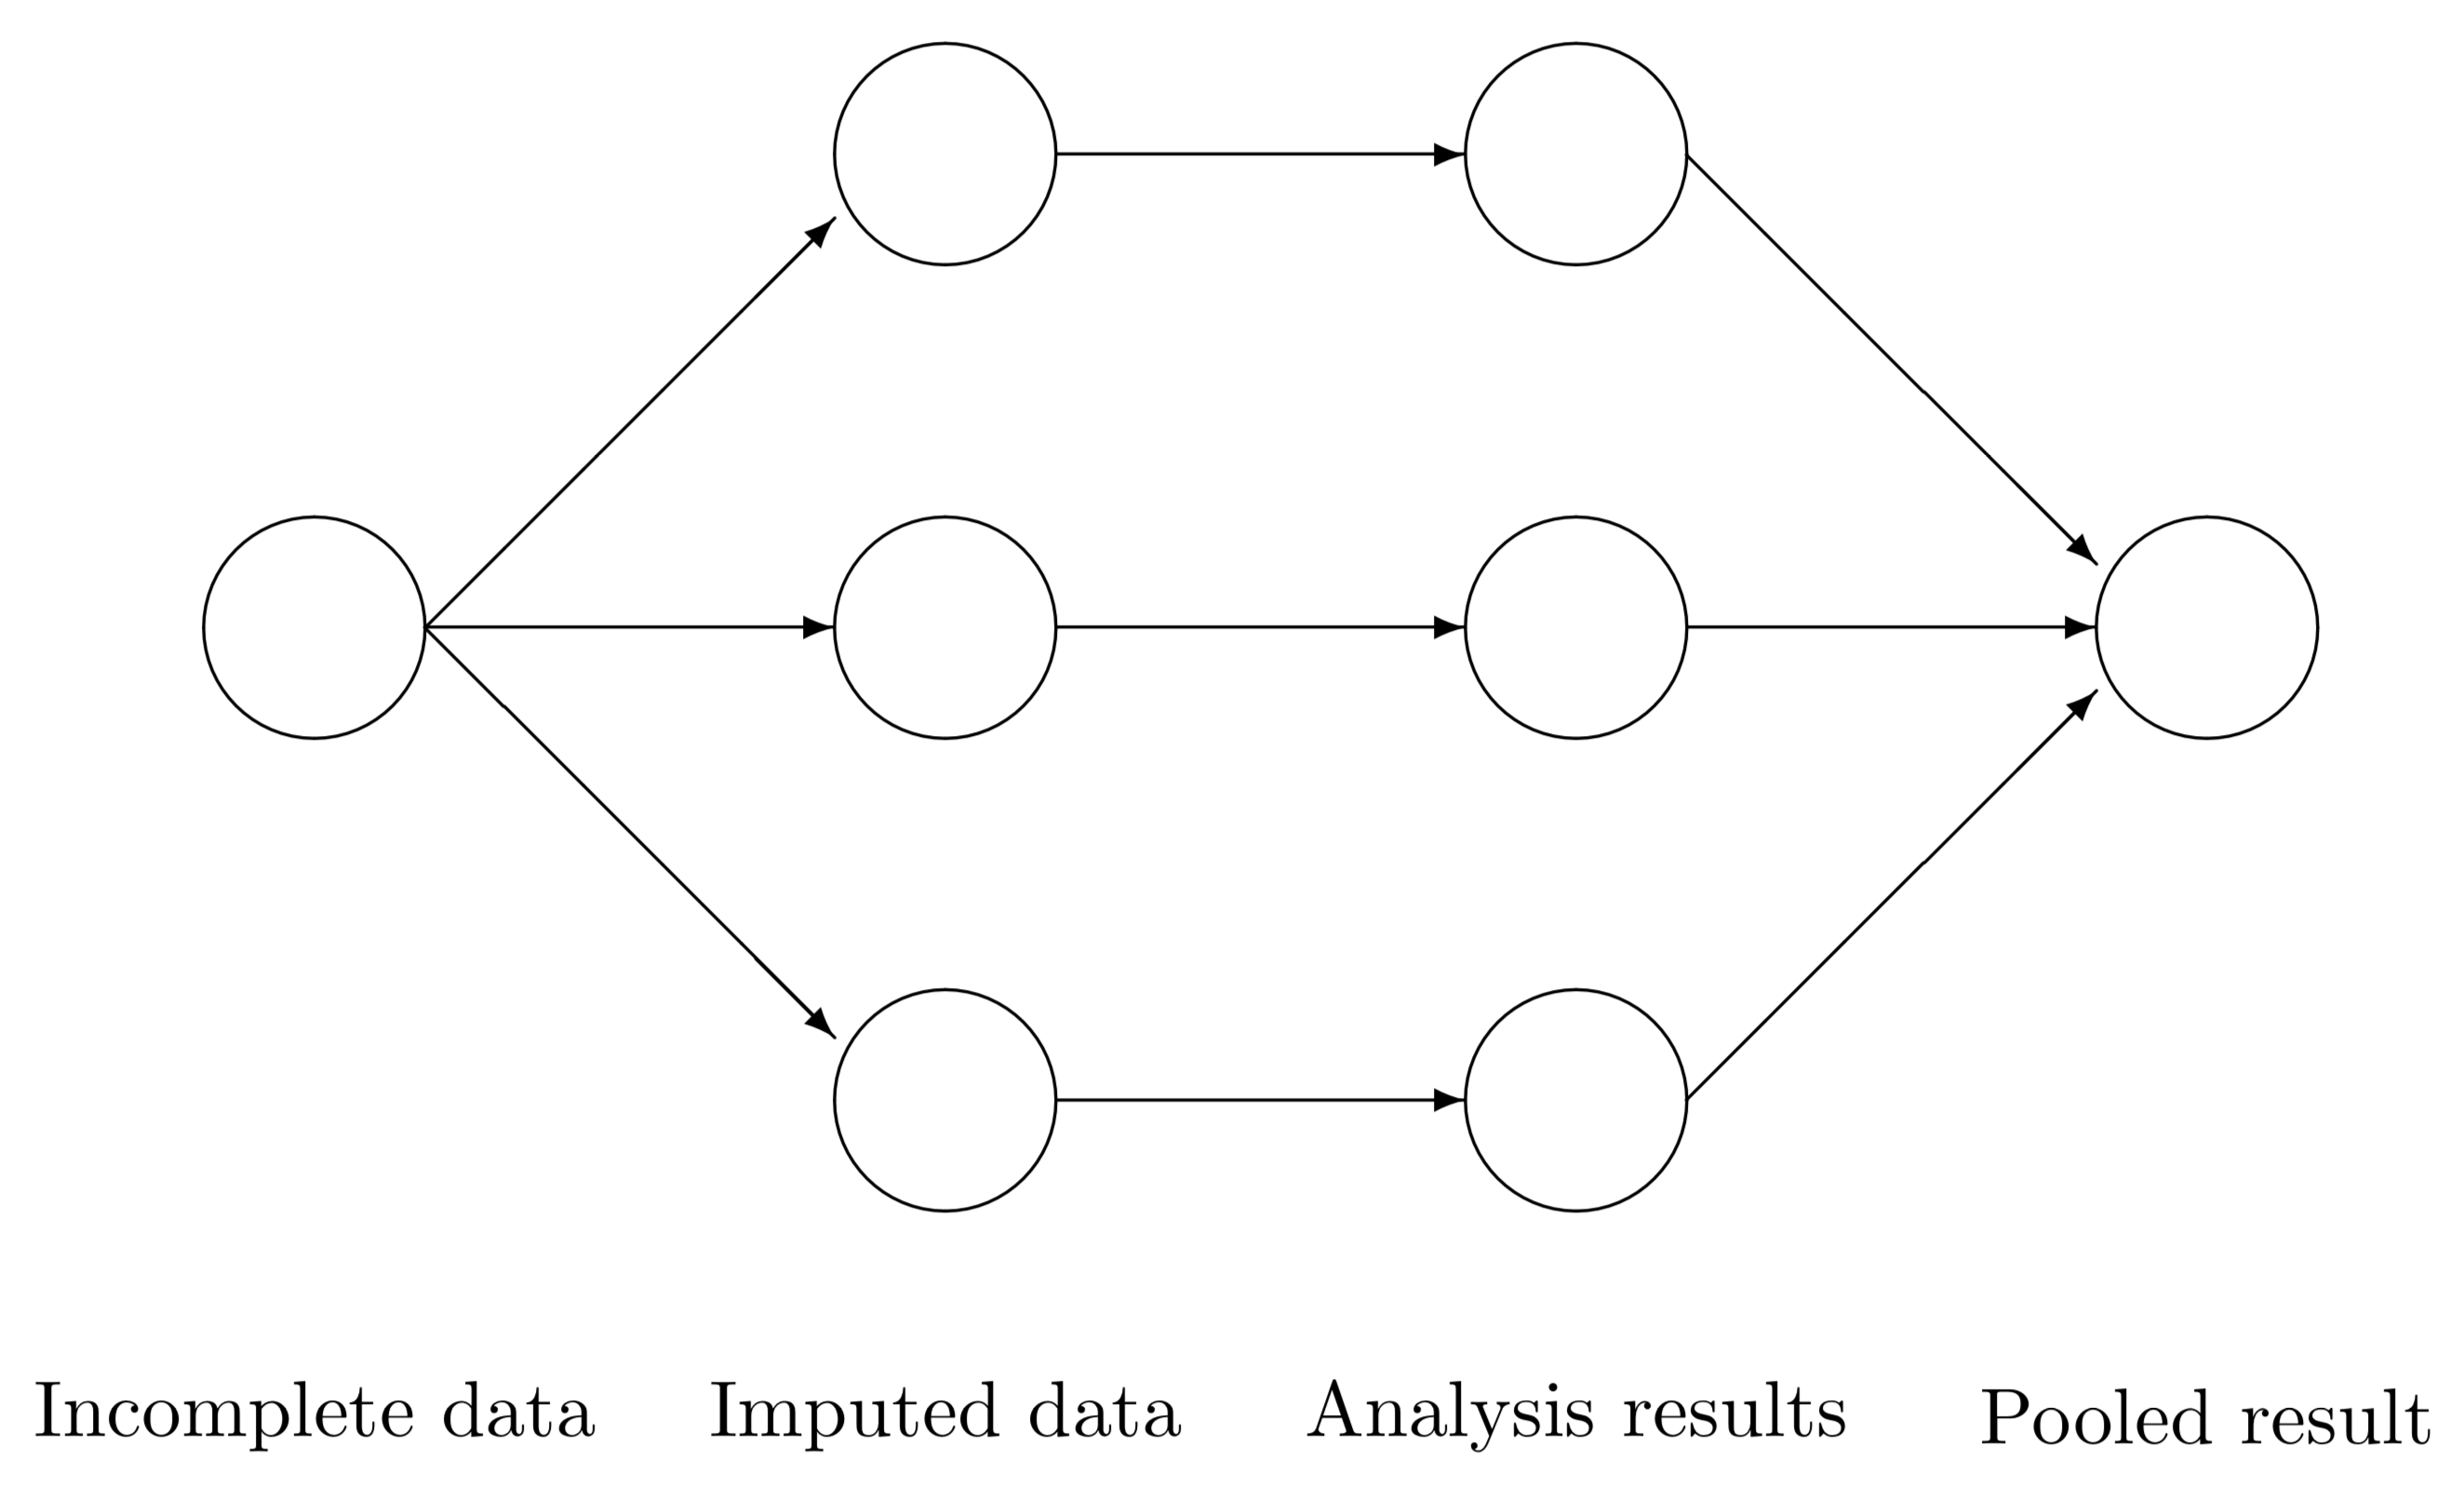
\includegraphics[scale=.2]{plots/miflow}
		\caption{Main steps used in \texttt{MICE} \citep{Buuren2011}}
		\label{fig6_1}
	\end{figure} 
	Figure \ref{fig6_1} illustrates how MICE solves a missing data problem by generating 3 imputed datasets. Three imputed datasets are generated with function \textbf{mice()}. Analysis are performed on every imputed dataset by \textbf{with()} function and combined into a single inference with function \textbf{pool()}. The software stores the output of each step in a particular class: \textbf{mids}, \textbf{mira} and \textbf{mipo}. More details about \texttt{MICE} package can be found in \citet{Buuren2011}.
	
	Two features of the software motivate our research. First, the default imputation method for numerical missing data is predictive mean matching (PMM) \citep{little1988missing}.
	\begin{lstlisting}
		library(mice, warn.conflicts = FALSE)
		imp <- mice(nhanes, print = FALSE)
		imp$method
	\end{lstlisting}
	\begin{verbatim}
		##   age   bmi   hyp   chl 
		##    "" "pmm" "pmm" "pmm"
	\end{verbatim}
	It generates imputations for a missing cell from its $p$ nearest points. The distance function applied to selection nearest points in MICE is:
	\begin{equation}
		\begin{array}{ll}
			d_{mice}(x_{i}^{obs}, x_{j}^{mis}) = |x_{i}^{obs}\beta^{*} - x_{j}^{mis}\hat{\beta}|,
		\end{array} 
	\end{equation}
	where $\hat{\beta}$ is the mean of the posterior distribution of models' parameters and $\beta^{*}$ is a random draw from the corresponding posterior distribution. Predictive mean matching is a non-parametric imputation approach that is proven to perform well in a wide range of scenarios \citep{de2011handbook, siddique2008multiple, su2011multiple, Buuren2018, Buuren2011, Vink2014, white2011multiple, Vink2015, yu2007evaluation}. The attractive advantage of PMM is that the imputed data is consistently within the range of the sample space \citep{heeringa2001multivariate, Buuren2018, Vink2014, Vink2015, white2011multiple, yu2007evaluation}. For instance, PMM prevents imputing negative values for data that are strictly non-negative. Second, \textbf{mids} only stores imputed datasets not the estimated parameters of the imputation models \citep{hoogland2020handling}. 
	
	Based on the features of \texttt{MICE} package discussed above, it is necessary to investigate whether PPC could check the donor selection procedure of PMM and perform PPC based on the observed data itself instead of the target statistics. \citet{he2012diagnosing} briefly discussed the approach to checking imputation models for subsets of missing variables. However, they assumed that the imputations of the remaining variables (excluding the incomplete variables of interest in an assessment) are adequate. Therefore, we also evaluate the performance of PPC when relaxing this assumption in the application section \ref{sec:6.6}.      
	
	The implement of PPC in \texttt{MICE} (version 3.13.15) is straightforward. A new argument \texttt{where} is included in \texttt{mice} function which allows us to replace the observed data by randomly drawing values from the predictive posterior distribution \citep{volker2021anonymiced}. Here is an example to generate replications of the observed data.   
	\begin{lstlisting}
		to_imp <- as.data.frame(!is.na(nhanes)) 
		imp <- mice(nhanes, where = to_imp, print = FALSE)
	\end{lstlisting}


	\section{Simulation Study}
	\label{sec:6.4}
	We carried out a simulation study to investigate the performance of the proposed diagnostic approach, varying several factors including missingness proportion (30\%, 50\%, 80\%), missingness mechanisms (MCAR and MARr), nominal levels of the confidence interval (75\%, 95\%) and different imputation models. The simulation study consisted of diagnostics under three scenarios: 1) quadratic equation with an incomplete outcome 2) quadratic equation with missing covariates 3) generalised linear model with an incomplete binary outcome. We evaluated whether the proposed diagnostic method could identify the congenial imputation model for continuous and discrete missing variables under the first and the third scenarios. We also investigated the performance of the proposed diagnostic method on the donor selection procedure of predictive mean matching under the second scenario. The sample size and the number of iterations were set to be 1000 and 50 separately in all simulations.  
	
	We induced missingness with the \texttt{ampute()} function in the simulation study. Generally, \texttt{ampute()} is a convenient function in \texttt{MICE} package to generate missing data for simulation purposes \citep{Schouten2018}. We considered missing completely at random (MCAR) mechanism where the probability of missingness is equal for every cell as well as right-tailed missing at random (MARr) mechanism where higher values of covariates have a higher probability of being unobserved. In the algorithm of \texttt{ampute()} function, the probability of missingness is allocated with different logistic functions of the weighted sum score, which is a linear combination of covariates correlated with the probability of missingness:
	\begin{equation}
		\begin{array}{ll}
			wss_{i} = w_{i}x_{1i} + w_{i}x_{2i} + \dots + w_{i}x_{mi}
		\end{array} 
	\end{equation}
	The weight $w_i$ is pre-specified to reflect the influence of the variable $x_{i}$ on the probability of missingness. For instance, if the formation of a weighted sum score is:
	$wss = x_1 + x_2$, the probability of missingness is determined by both $x_1$ and $x_2$ with the equal effects. More specifically, under MARr mechanism, candidates with higher values of weighted sum score have a higher probability of being unobserved when applying the \texttt{ampute()} function to generate missing data.
	
	\subsection{Quadratic equation with an incomplete outcome}
	In the first simulation study, we considered a partially observed variable $Y$ and a fully observed variable $X$. The data was generated from : $X \sim unif(-3, 3)$, $Y|X \sim \mathcal{N}(X + X^2, 1)$. The scientific model was indeed a quadratic model. We considered two imputation models for the missing response $Y$: one is a linear regression of $Y$ on $X$, and the other is a quadratic regression of $Y$ on $X$. 
	
	\subsection{Quadratic equation with incomplete covariates}
	In the second simulation study, the response variable $Y$ was generated from a normal distribution: $Y|X \sim \mathcal{N}(X + X^2, 1)$, where the covariate $X$ followed a standard normal distribution. In this simulation study, the response variable $Y$ was completely observed while the covariate $X$ and the corresponding quadratic term $X^2$ were jointly missing for a part of the cases. There were no cases with missing cells on either $X$ or $X^2$. We compared two non-parametric methods, predictive mean matching (PMM) and polynomial combination (PC) with a parametric method, the substantive model compatible fully conditional specification (SMC-FCS) \citep{Vink2013, bartlett2015multiple}. The PC and SMC-FCS methods are two accepted methods to impute linear regression with quadratic terms. The PC method is an extension of PMM but applies a different donor selection procedure. 
	
	\subsection{Generalised linear model for discrete variables}
	The final simulation study considered a partially observed binary $Y$ and two complete covariates $X$ and $Z$. The model of scientific interest was : $Pr (Y = 1 | X, Z) = exp(X + Z) / 1 + exp(X + Z)$,
	where $x \sim unif(-3 , 3)$ and $Z \sim \mathcal{N}(1, 1)$. Under MARr mechanism, the weights of variables $X$ and $Z$ in determining the probability of missingness for $Y$ were set to be equal. Since the logistic regression actually models the probability of assignment, we investigated the plot of deviance and calculated the sum of squared deviance divided by the sample size. There were two candidate models: a logistic regression of $Y$ on $X$ and $Z$ and a logistic regression of $Y$ on $Z$ only.
	
	\section{Simulation results}
	\label{sec:6.5}
	In this section, we present the simulation results of the proposed diagnostic method under three different scenarios. For numerical assessment, we estimated the rate by which the confidence interval covers the observed data (COV), the mean of the distance between the observed data and the mean of corresponding predictive posterior distributions (Distance), and the average width of the confidence intervals (CIW). We also provided graphical analyses with scatterplots, density plots, and distribution plots, which show observed values, upper and lower bounds of confidence intervals for each observed data point. Sometimes a single plot or summarised statistic is inadequate to arrive at a conclusion. Conducting PPC with various tools would provide a more comprehensive evaluation of the imputation model.     
	
	\subsection{Quadratic equation with an incomplete outcome}
	Table \ref{tab6_1} shows the results of the simulation study when the substantive model is a quadratic equation with an incomplete outcome. Since we only generated one incomplete dataset and repeated imputing it 50 times, all coverage rates were close to the pre-specified nominal level. However, when the imputation model was misspecified as a linear regression model, the average distance was larger than the average distance under the correct specification of the imputation model (linear regression with a quadratic term). It conforms to our intuitive idea that the data would be close to the centre of predictive posterior distributions if the model fits. The variance of the missing variable $Y$ was set as 1, which implied that the width of 95\% nominal confidence interval is approximate 3.92 ($1.96 \times 2$) and the width of 75\% nominal confidence interval is approximate 2.3 ($1.15 \times 2$). When the imputation model was correctly specified, the estimated average width of the confidence interval was unbiased. However, the variance of $Y$ was overestimated when the imputation model was linear. 
	
	The same result could also be derived from the graphical analysis. Figure \ref{fig6_2} shows distribution plots under the scenario of 30\% missing cases and MARr missing mechanism. This plot provides upper and lower bounds of the posterior predictive distribution for all observed $Y$ in ascending order of the mean of the posterior distribution. Green points imply the corresponding observed value falls in the interval, while red points imply the corresponding observed value falls out the interval. 
	
	When the imputation model was correctly specified, the points out of the 95\% confidence interval were randomly spread over the sample space without any patterns. However, when the imputation model was incorrectly specified as the linear regression model, the points out of the confidence interval clustered in the regions with extreme values of $X$. Moreover, the width of the intervals was generally narrower when the model was correct. The density plot and the scatter plot of the observed and replicated data generated with function \textbf{densityplot()} and \textbf{xyplot()} in \texttt{MICE} also show the evidence that the quadratic regression is preferable than the linear model (see figure \ref{fig6_3}). The scatter plot of the quadratic regression imputation model shows that replicated data overlapped the observed data. The density plot shows that the replicated data shared the same distribution as the observed data. This evidence illustrates the congeniality of the quadratic regression imputation model. However, the linear regression model performed worse than the quadratic regression model. First, the replicated data did not cover the observed data in two extreme regions in the scatter plot. Second, the empirical density of the replicated data and observed data were different. 
	
	These three plots do not merely illustrate the misspecification of the imputation model as the linear regression model. They also provide information to identify the regions of sample space in which the sub-optimal imputation model could still generate acceptable imputed values. Based on the distribution plot for the linear regression imputation model, we could also develop the piecewise linear regression model for the observed data. 
	
	When we cannot figure out the imputation model under which the observed data fit the predictive posterior distribution perfectly, these plots based on observed data provide the evidence of rebuilding a piecewise imputation model, which would improve the validity of imputation values. When the missing cases are not in the regions where outliers crowd, we could even apply the uncongenial imputation model. For example, in our simulation scenario, suppose we only consider the linear regression imputation model and missing cases with near parabolic minimum $X$ values. The imputed value will not show significant deviations from the true value. Finally, our proposed PPC approach for imputation models is robust against the different percentages of missing cases, missingness mechanisms, and the confidence interval's nominal levels. The nominal level of the confidence interval is determined by the extent to which we could undertake the outliers when the imputation model is not congenial with the data generating process. For instance, there were more outliers in the plot of means and 75\% confidence intervals than the plot of mean and 95\% confidence intervals. When we would like to replace the linear regression model with a piecewise linear model to improve the imputation, the selection knots based on the 75\% confidence intervals are more closed to the parabolic minimum than the 95\% confidence intervals (See figure \ref{fig6_4}). 
	
	\subsection{Quadratic equation with incomplete covariates}	
	Table \ref{tab6_2} and \ref{tab6_3} show the result of the simulation for the quadratic equation with incomplete covariates. Based on the numerical results, the performance of these three methods, PC, SMC-FCS, and PMM, was the same, despite the slightly reduced coverage rate of PMM. In fact, when the missingness mechanism is MCAR (to bypass the problem of the sparse observed region for PMM), PMM would also provide a valid inference of the regression parameters (see Table \ref{tab6_4}) \citep{Vink2013}.
	
	However, when it comes to graphical diagnostics, the misfit of PMM appears. The distribution plot (figure \ref{fig6_5} and \ref{fig6_6}) show that PC and SMC-FCS generated the same posterior predictive distribution of the observed data. There were more outliers with a larger value of $Y$. It is sensible since the density function of $X$ based on $Y$ is not monotone. Thus, it is unavoidable to impute the missing cell on the opposite arm of the parabolic function. Although in such a case, the imputed value was not the same as the true value, the replicated data still overlapped the observed data in the scatter plot (see Figures \ref{fig6_7}). The distribution plot of PMM with a 95\% nominal level in Figure \ref{fig6_5} did not show more outliers than these of PC and SMF-FCS. However, when the nominal level was set to 75\%, more outliers appeared in the sub-plot of PMM (Figure \ref{fig6_6}). The reason is that there are more observed data closed to the centre in the plots of PC and SMC-FCS, which implies the superiority of PC and SMC-FCS. The scatter plot also shows the discrepancy between the distribution of the replicated and the observed data with respect to PMM (Figures \ref{fig6_7}). The result is robust against various percentages of missing cases and over the studied missing mechanisms. The proposed PPC for the imputation model could check the donor selection process of hot-deck approaches. In our simulation scenarios, selecting donors for the composition $X + X^2$ performed better than only solving for the missing variable $X$. SMC-FCS was treated as the baseline in our simulation since it is proven as a reliable imputation method when the substantive model is known \citep{bartlett2015multiple}. The PC performs as well as the SMC-FCS which implies the donor selection process of PC reflects the data generating process in our simulation scenarios. However, when applying hot-deck approaches to implement imputation, the success in model checking is not sufficient to define valid imputations. In order to determine whether we could derive plausible imputations, additional diagnoses of distribution of the complete variable for observed and missing cases are necessary. For example, in our simulation scenario, if the variable $Y$'s range of missing cases is out of the range of observed cases, the PC may still derive implausible imputations. 
	
	\subsection{Generalised linear model for discrete variables}
	Table \ref{tab6_5} shows the average sum of squared deviance for two different logistic regression models. The value of the average sum of squared deviance was smaller when the imputation model was correctly specified with logistic regression on both $X$ and $Z$. The result is robust against the percentage of missing cases and missingness mechanisms. Figure \ref{fig6_8} shows that the residuals tend to zero when the imputation model fits the observed data better. The distribution of the observed data was more extreme than the empirical posterior distributions of replicated data generated under the logistic model with only variable $Z$. 
	
	\section{Application}
	\label{sec:6.6}
	\subsection{Background}
	We illustrate the application of the proposed PPC for multiple missing variables with the data from the body mass index (BMI) of the Dutch. This application is to study whether the proposed PPC works for a sequence of imputation models. More specifically, we aim to investigate whether the incorrect imputation model for one missing variable would disturb the proposed PPC for other variables. BMI is defined as the body weight divided by the square of the body height, which is broadly applied to categorise a person into underweight, normal, overweight, and obese. Since measuring a person's weight and height is costly, an alternative is to ask people to report their weight and height. However, such self-report data is systematically biased. People are used to overestimating their height and underestimating their weight, leading to a lower self-report BMI compared with measured BMI \citep[Section 9.3]{Buuren2018}. The goal of the study is to estimate unbiased BMI from the self-report data. We apply the multiple imputation approach to fill the unobserved measured weight and height. 
	
	The data we analyze is named \texttt{selfreport} in \texttt{MICE} package. The data consists of two components. One is the calibration dataset that contains 1257 Dutch individuals with both self-report and measured height and weight and was taken from \citet{krul2011self}. The original survey measured 4459 adults in either Italy, Netherlands, or North America aged 18-65 years in 1999 or 2000. The second part is the survey dataset containing 803 Dutch adults aged 18-75 years with only self-reported data. The survey data were collected in November 2007, either online or using paper-and-pencil methods \citep[Section 9.3]{Buuren2018}. Six variables are included in the application: \texttt{age} (years), \texttt{sex} (male or female), \texttt{hm} denoting measured height (cm), \texttt{hr} denoting self-reported height (cm), \texttt{wm} denoting measured weight (kg), and \texttt{wr} denoting self-reported weight (kg). 
	
	To fit the aim of this application study, we design two linear regression imputation models for \texttt{hm}: one includes all the other variables, and the other includes all the other variables except the variable \texttt{hr}. Similarly, there are two linear regression imputation models for \texttt{wm}: one includes all the other variables, and the other includes all the other variables except the variable \texttt{wr}. In such a case, we have four imputation strategies to evaluate:
	\begin{enumerate}
		\item Case 1: include \texttt{hr} in the imputation model of \texttt{hm} and \texttt{wr} in the imputation model of \texttt{wm}.
		\item Case 2: include \texttt{hr} in the imputation model of \texttt{hm} and exclude \texttt{wr} from the imputation model of \texttt{wm}.
		\item Case 3: exclude \texttt{hr} from the imputation model of \texttt{hm} and include \texttt{wr} in the imputation model of \texttt{wm}.
		\item Case 4: exclude \texttt{hr} from the imputation model of \texttt{hm} and \texttt{wr} from the imputation model of \texttt{wm}.
	\end{enumerate}
	Although it is evident that \texttt{hr} and \texttt{wr} are significant covariates for the imputation of \texttt{hm} and \texttt{wm}, we deliberately ignore these two variables in some cases to evaluate whether incorrect imputation model for \texttt{hm} (\texttt{wm}) influences PPC for \texttt{wm} (\texttt{hm}).
	 
	\subsection{Results}
	Table \ref{tab6_6} shows that the best imputation model among these four is the one that includes both \texttt{wr} and \texttt{hr}. The average distance and the width of confidence intervals for the observed data were the smallest for both \texttt{hm} and \texttt{wm}. No matter the imputation model of \texttt{hm} was correctly specified, the linear regression imputation model for \texttt{wm} should be based on all the other variables. When fixing the imputation model for the \texttt{hm} (no matter including \texttt{hr} or not), the average distance and the average width of the confidence interval of \texttt{hm} derived under the linear model included \texttt{hr} was remarkably less than the result taken under the linear model excluded the covariate \texttt{hr}. The graphical results (Figure \ref{fig6_9}-\ref{fig6_12}) show the same conclusion. When the linear regression imputation model for \texttt{wm} or \texttt{hm} was correctly specified, the imputed data overlapped the observed data in the scatter plot. The observed data would be closer to the centre of the confidence interval, and the width of confidence intervals was relatively small. However, the result of \texttt{wr} in case 3 was slightly larger than that in case 1. Similarly, the result of \texttt{wr} in case 4 was slightly larger than that in case 2. A similar result could be found in fixing the imputation model for the \texttt{wm} (no matter the imputation model includes \texttt{wr} or not). The average distance and the average confidence interval of \texttt{wm} derived under the linear model had \texttt{wr} was remarkably less than the result taken under the linear model excluded the covariate \texttt{wr}.
	
	The findings imply that incorrect specification of the imputation models for other missing variables $Y_{-j}$ would influence the target variable $Y_j$ for which we perform the PPC because densities of the imputed variables $Y_{-j}$ are different from the `true' densities. However, we can still select the correct model for $Y_j$. Our application scenario is relatively simple: the linear model is sufficient to reflect the data generating process of missing variables. However, we do not rule out the possibility that under extreme and complicated cases, incorrect specification of the imputation models for other missing variables $Y_{-j}$ would prevent us from selecting the most suitable imputation model for the missing variable $Y_j$. 
	
	\section{Discussion}
	\label{sec:6.7}
	The proposed imputation model diagnostic procedure based on PPC involves numerical assessment and graphical analysis. For numerical assessment, the evidence of a fitted imputation model is less deviation between the observed value and the expectation of corresponding predictive posterior distribution and narrower width of confidence intervals of predictive posterior distributions for the observed data. For graphical analysis, we provide the distribution plot, the scatter plot and the density plot. The more suitable imputation models are, the more similar the replicated data to the observed data in the density and scatter plots. The distribution plot shows posterior distributions of all observed data. It allows the researcher to identify the regions where the imputation model misfits. It is noteworthy that applying both numerical and graphical tools benefits a thorough understanding of model selection.
	
	The simulation study demonstrates that the proposed imputation model diagnostic procedure works on continuous and discrete variables under parametric and hot-deck multiple imputation approaches. We could derive more information for a continuous variable, such as the way to improve the imputation model, because of the distribution plot. For example, although the imputation model is incorrect in general, it provides valid imputations in the focused regions. In such a case, we could still apply the suboptimal imputation model. Moreover, we could only adjust the imputation model in the misfitted regions and develop a piecewise imputation model. The PPC for categorical data or ordered categorical data is limited, since the predictor of the imputation model is the probability of assignment rather than the observed data itself. We currently investigate residual deviance as the indicator to select the model for categorical data and ordered categorical data. For hot-deck imputation approaches, what PPC diagnoses is the donor-selection procedure. However, based on the features of predictive mean matching, the appropriate donor selection does not ensure plausible imputations. Extra analysis of the observed data and the imputed data is necessary.   
	
	The application example shows that the PPC works on the multivariate missing datasets. When the imputed covariate deviates from the actual distribution because of the mis-specified imputation models, the imputation model for the predictor could also be selected by PPC. In our case study, the misspecification of one missing variable slightly influences the other missing variable's numerical results. However, in more extreme situations, such as a large number of missing variables and more ridiculous imputation models for covariates, the result may be influenced seriously, so as to result in a sub-optimal model selection. Therefore, it is more reasonable to perform the numerical analysis of all missing variables and make the model selection for those variables with remarkably different results under different candidate imputation approaches first. 
	
	Existing PPC proposed by \citet{he2012diagnosing} and \citet{gelman2005multiple} measured the posterior predictive p-value to indicate the discrepancies of summarised statistics between the observed and replicated data. The close to 0 or 1 p-value implies the inadequacy of the imputation model with respect to the target quantities. The target quantities should be calculated with the completed data, which consists of the observed and the imputed data because it allows the researcher to calculate the target quantities requiring a complete data matrix. Both \citet{he2012diagnosing} and \citet{nguyen2015posterior} found that the existing PPC for multiple imputation model is sensitive to the percentage of missing cases. Since the imputed and replicated data are generated from the same posterior predictive distribution, the diagnostic becomes more difficult with an increasing proportion of missing data.
	
	Unlike the existing PPC approach, the PPC discussed in the paper checks the imputation model for each missing variable under the FCS framework. We diagnose the distribution of the observed data so that the result would also be reliable with a large proportion of missing cases. The simulation study also shows that the proposed PPC works for different missingness mechanisms. The PPC for multiple imputation models based on target analysis would be more informative when the imputer is also the researcher. The issue would be whether a valid inference for the scientific interest could be derived from the imputed data. However, the PPC for multiple imputation models based on the observed data addresses another issue: whether the imputation model is congenial to the substantive model. The imputed data generated after the proposed PPC could be used for more general downstream analysis and different scientific interests.
	
	When the sample size is tremendous, it is better to choose some representative data to check the imputation model so that the scatter plot or the distribution plot would not be too crowded. A clustered procedure could be applied to gather the observed data with closed values and choose one subset in each cluster to check the model. Further investigation is necessary to set the rule to select the observed data when the sample size is too large.
	
	\newpage
	\begin{sidewaystable}[ht!]
		\begin{tabular}{cc|cccc|cccc|cccc}
			\multicolumn{2}{l|}{}                             & \multicolumn{4}{c|}{COV}                                                                                           & \multicolumn{4}{c|}{Average Distance}                                                                              & \multicolumn{4}{c}{Average CIW}                                                                                   \\ \cline{3-14} 
			\multicolumn{1}{l}{}      & \multicolumn{1}{l|}{} & \multicolumn{2}{c}{linear model}                        & \multicolumn{2}{c|}{quadratic model}                     & \multicolumn{2}{c}{linear model}                        & \multicolumn{2}{c|}{quadratic model}                     & \multicolumn{2}{c}{linear model}                        & \multicolumn{2}{c}{quadratic model}                     \\ \hline
			\multicolumn{1}{l|}{}     & \multicolumn{1}{l|}{} & \multicolumn{1}{l}{75\%CI} & \multicolumn{1}{l}{95\%CI} & \multicolumn{1}{l}{75\%CI} & \multicolumn{1}{l|}{95\%CI} & \multicolumn{1}{l}{75\%CI} & \multicolumn{1}{l}{95\%CI} & \multicolumn{1}{l}{75\%CI} & \multicolumn{1}{l|}{95\%CI} & \multicolumn{1}{l}{75\%CI} & \multicolumn{1}{l}{95\%CI} & \multicolumn{1}{l}{75\%CI} & \multicolumn{1}{l}{95\%CI} \\
			\multicolumn{1}{c|}{}     & missingness           &                            &                            &                            &                             &                            &                            &                            &                             &                            &                            &                            &                            \\ \cline{2-14} 
			\multicolumn{1}{c|}{}     & 30                    & 0.76                       & 0.96                       & 0.75                       & 0.93                        & 2.41                       & 2.41                       & 0.79                       & 0.79                        & 6.64                       & 11.32                      & 2.27                       & 3.87                       \\
			\multicolumn{1}{c|}{MCAR} & 50                    & 0.72                       & 0.96                       & 0.76                       & 0.94                        & 2.44                       & 2.44                       & 0.77                       & 0.77                        & 6.61                       & 11.27                      & 2.25                       & 3.83                       \\
			\multicolumn{1}{c|}{}     & 80                    & 0.77                       & 0.95                       & 0.78                       & 0.94                        & 2.25                       & 2.25                       & 0.87                       & 0.87                        & 6.53                       & 11.13                      & 2.51                       & 4.28                       \\\hline
			\multicolumn{1}{c|}{}     & 30                    & 0.75                       & 0.95                       & 0.74                       & 0.94                        & 2.28                       & 2.28                       & 0.8                        & 0.8                         & 6.26                       & 10.66                      & 2.31                       & 3.94                       \\
			\multicolumn{1}{c|}{MARr} & 50                    & 0.76                       & 0.95                       & 0.73                       & 0.95                        & 2.21                       & 2.21                       & 0.81                       & 0.81                        & 6.3                        & 10.73                      & 2.3                        & 3.91                       \\
			\multicolumn{1}{c|}{}     & 80                    & 0.8                        & 0.96                       & 0.77                       & 0.92                        & 1.8                        & 1.8                        & 0.83                       & 0.83                        & 5.43                       & 9.25                       & 2.38                       & 4.05                      
		\end{tabular}
		\caption{The rate of nominal confidence interval covers the observed data (COV), the mean of the distance between the observed data and the location of the predictive posterior distribution (Distance), and the average width of the nominal (75\% and 95\%) confidence intervals (CIW) for two imputation models (linear model and quadratic model) under different combinations of experimental factors. The analysis model is a quadratic equation.}
		\label{tab6_1}
	\end{sidewaystable}
	
	\begin{sidewaystable}[ht!]
		\begin{tabular}{cc|ccc|ccc|ccc}
			\multicolumn{2}{l}{}                    & \multicolumn{3}{c|}{COV} & \multicolumn{3}{c|}{Average distance} & \multicolumn{3}{c}{Average CIW} \\ \cline{2-11} 
			\multicolumn{1}{c|}{}     & missingness & PC    & SMC-FCS  & PMM   & PC         & SMC-FCS      & PMM       & PC       & SMC-FCS    & PMM     \\
			\multicolumn{1}{c|}{}     & 30          & 0.94  & 0.94     & 0.91  & 0.62       & 0.62         & 0.68      & 3.02     & 3.1        & 3.03    \\
			\multicolumn{1}{c|}{MCAR} & 50          & 0.94  & 0.93     & 0.9   & 0.61       & 0.61         & 0.67      & 3.03     & 3.06       & 2.97    \\
			\multicolumn{1}{c|}{}     & 80          & 0.96  & 0.94     & 0.91  & 0.61       & 0.64         & 0.65      & 3.06     & 3.14       & 3       \\ \hline
			\multicolumn{1}{c|}{}     & 30          & 0.94  & 0.94     & 0.89  & 0.59       & 0.59         & 0.64      & 2.93     & 2.84       & 2.84    \\
			\multicolumn{1}{c|}{MARr} & 50          & 0.93  & 0.94     & 0.89  & 0.57       & 0.58         & 0.62      & 2.74     & 2.7        & 2.68    \\
			\multicolumn{1}{c|}{}     & 80          & 0.93  & 0.97     & 0.93  & 0.56       & 0.56         & 0.61      & 2.61     & 2.64       & 2.69   
		\end{tabular}
		\caption{The rate of nominal confidence interval covers the observed data (COV), the mean of the distance between the observed data and the location of the predictive posterior distribution (Distance), and the average width of the nominal 95\% confidence intervals (CIW) for PC, SMC-FCS and PMM under different combinations of experimental factors. The analysis model is a quadratic equation.}
		\label{tab6_2}
	\end{sidewaystable}
	
	\begin{sidewaystable}[ht!]
		\begin{tabular}{cc|ccc|ccc|ccc}
			\multicolumn{2}{l}{}                    & \multicolumn{3}{c|}{COV} & \multicolumn{3}{c|}{Average distance} & \multicolumn{3}{c}{Average CIW} \\ \cline{2-11} 
			\multicolumn{1}{c|}{}     & missingness & PC    & SMC-FCS  & PMM   & PC         & SMC-FCS      & PMM       & PC       & SMC-FCS    & PMM     \\
			\multicolumn{1}{c|}{}     & 30          & 0.76  & 0.75     & 0.7   & 0.62       & 0.62         & 0.68      & 1.77     & 1.82       & 1.78    \\
			\multicolumn{1}{c|}{MCAR} & 50          & 0.75  & 0.75     & 0.73  & 0.61       & 0.61         & 0.67      & 1.78     & 1.8        & 1.74    \\
			\multicolumn{1}{c|}{}     & 80          & 0.78  & 0.76     & 0.75  & 0.61       & 0.64         & 0.65      & 1.8      & 1.84       & 1.76    \\ \hline
			\multicolumn{1}{c|}{}     & 30          & 0.76  & 0.74     & 0.71  & 0.59       & 0.59         & 0.64      & 1.72     & 1.66       & 1.67    \\
			\multicolumn{1}{c|}{MARr} & 50          & 0.74  & 0.72     & 0.69  & 0.57       & 0.58         & 0.62      & 1.61     & 1.58       & 1.57    \\
			\multicolumn{1}{c|}{}     & 80          & 0.75  & 0.73     & 0.7   & 0.56       & 0.56         & 0.61      & 1.53     & 1.55       & 1.58   
		\end{tabular}
		\caption{The rate of nominal confidence interval covers the observed data (COV), the mean of the distance between the observed data and the location of the predictive posterior distribution (Distance), and the average width of the nominal 75\% confidence intervals (CIW) for PC, SMC-FCS and PMM under different combinations of experimental factors. The analysis model is a quadratic equation.}
		\label{tab6_3}
	\end{sidewaystable}
	
	\begin{table}[ht!]
		\begin{tabular}{cccc}
			& True value & Estimates value & Coverage rate \\
			$\beta_1$ & 1          & 1.008           & 0.934         \\
			$\beta_2$ & 1          & 1               & 0.958        
		\end{tabular}
		\caption{The PMM performs under the scientific model : $Y = \alpha + X\beta_{1} + X^2\beta_{2} +\epsilon$, where $\alpha = 0$, $\beta_{1} = 1$ and $\beta_{2} = 1$. The error term and variable $X$ follow standard normal distributions. 30\% cases of $X$ and $X^2$ are designed to be jointly missing. The missingness mechanism is MCAR.}
		\label{tab6_4}
	\end{table}
	
	\begin{table}[ht!]
		\begin{tabular}{cc|cc}
			&             & \multicolumn{2}{c}{mean of residual deviance} \\ \cline{2-4} 
			\multicolumn{1}{c|}{}     & missingness & with x               & without x               \\
			\multicolumn{1}{c|}{}     & 30          & 0.83                 & 1.25                    \\
			\multicolumn{1}{c|}{MCAR} & 50          & 0.85                 & 1.27                    \\
			\multicolumn{1}{c|}{}     & 80          & 0.95                 & 1.3                     \\ \hline
			\multicolumn{1}{c|}{}     & 30          & 0.9                  & 1.34                    \\
			\multicolumn{1}{c|}{MARr} & 50          & 0.94                 & 1.35                    \\
			\multicolumn{1}{c|}{}     & 80          & 0.98                 & 1.28                   
		\end{tabular}
		\caption{The average sum of squared deviance for two imputation models: 1) logistic regression with two predictors $x$ and $z$ 2) logistic regression with one predictor $x$ under different combinations of experimental factors. The outcome is a dichotomous variable $y$ and the binary regression is based on $x$ and $z$.}
		\label{tab6_5}
	\end{table}
	
	\begin{table}[ht!]
		\begin{tabular}{c|ccc|ccc}
			& \multicolumn{3}{c|}{hm}               & \multicolumn{3}{c}{wm}                \\ \cline{2-7} 
			& cov  & average distance & average CIW & cov  & average distance & average CIW \\
			strategy 1 & 0.95 & 1.57             & 8.27        & 0.95 & 2.28             & 12.46       \\
			strategy 2 & 0.95 & 1.65             & 8.89        & 0.94 & 10.9             & 54.38       \\
			strategy 3 & 0.95 & 5.58             & 26.89       & 0.94 & 2.35             & 12.83       \\
			strategy 4 & 0.95 & 5.56             & 27.88       & 0.97 & 9.84             & 59.57      
		\end{tabular}
		\caption{The performance of 4 imputation strategies is summarised by the coverage rate, the average distance and the average width of confidence intervals with respect to missing variables \texttt{hm} and \texttt{wm}}
		\label{tab6_6}
	\end{table}
	
	\newpage
	\begin{figure}[b]
		\begin{center}
			\resizebox{\textwidth}{!}{
				\subfigure[quadratic imputation model]{
					\label{boxplot:a}
					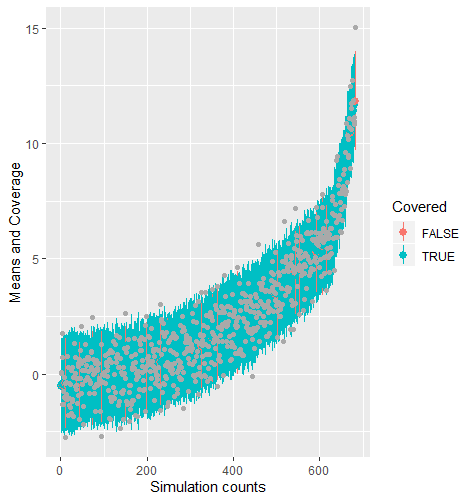
\includegraphics[scale=.5]{plots/plot6.1}
				}
				\subfigure[linear imputation model]{
					\label{boxplot:b}
					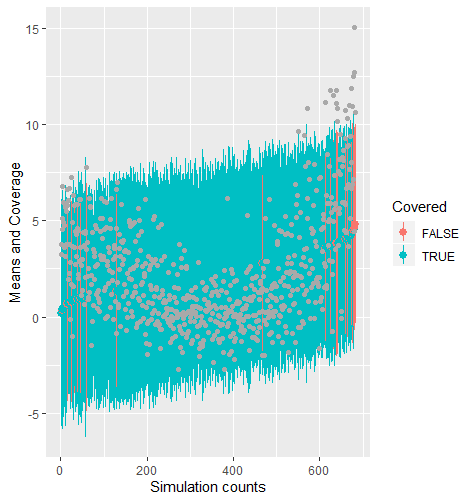
\includegraphics[scale=.5]{plots/plot6.2}
				}
			}
		\end{center}
		\caption{Distribution plots for the first simulation study (quadratic equation with an incomplete outcome) generated under 30\% missing cases and MARr missingness mechanism. The confidence interval is 95\% nominal.}
		\label{fig6_2}
	\end{figure}
	
	\begin{figure}[ht!]
		\begin{center}
			\resizebox{\textwidth}{!}{
				\subfigure[quadratic imputation model]{
					\label{boxplot:a}
					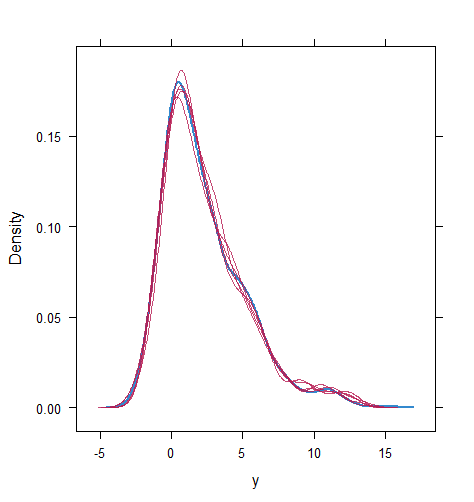
\includegraphics[scale=.5]{plots/plot6.3}
				}
				\subfigure[linear imputation model]{
					\label{boxplot:b}
					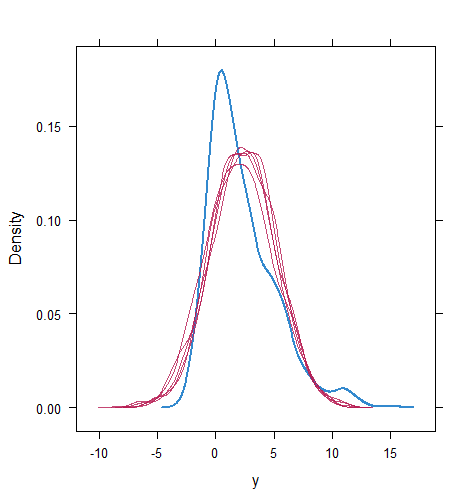
\includegraphics[scale=.5]{plots/plot6.4}
				}
			}\\ 	
			\resizebox{\textwidth}{!}{
				\subfigure[quadratic imputation model]{
					\label{boxplot:c}
					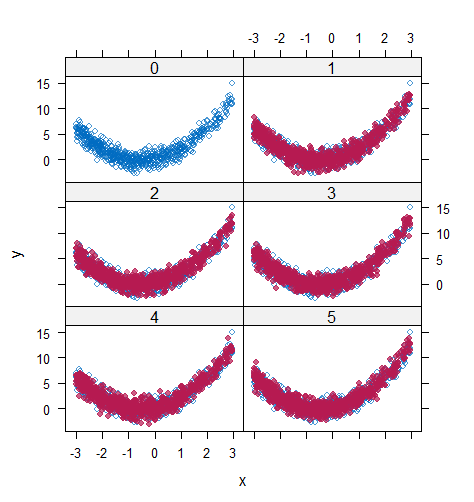
\includegraphics[scale=.5]{plots/plot6.5}
				}
				\subfigure[linear imputation model]{
					\label{boxplot:d}
					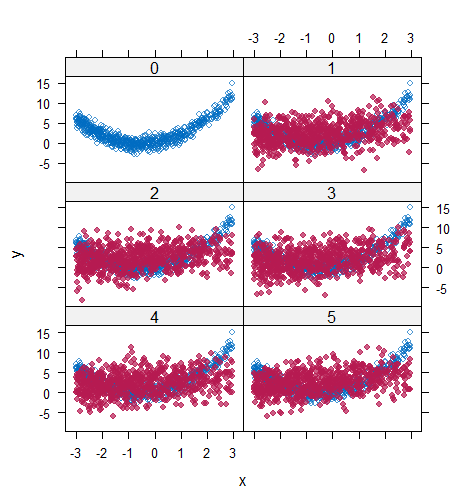
\includegraphics[scale=.5]{plots/plot6.6}
				}
			}
		\end{center}
		\caption{Scatterplots and densityplots for the first simulation study (quadratic equation with an incomplete outcome) generated under 30\% missing cases and MARr missingness mechanism.}
		\label{fig6_3}
	\end{figure}
	
	\begin{figure}[ht!]
		\begin{center}
			\resizebox{\textwidth}{!}{
				\subfigure[quadratic imputation model]{
					\label{boxplot:a}
					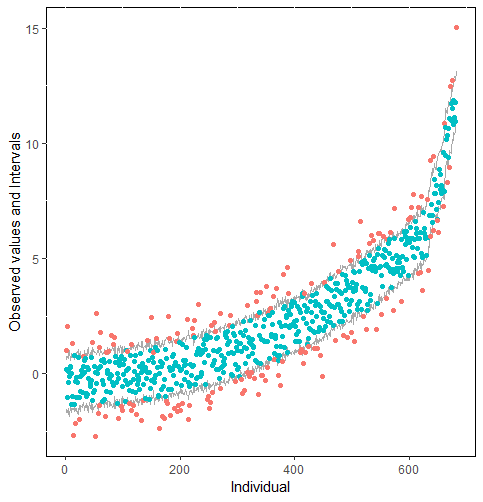
\includegraphics[scale=.5]{plots/plot6.7}
				}
				\subfigure[linear imputation model]{
					\label{boxplot:b}
					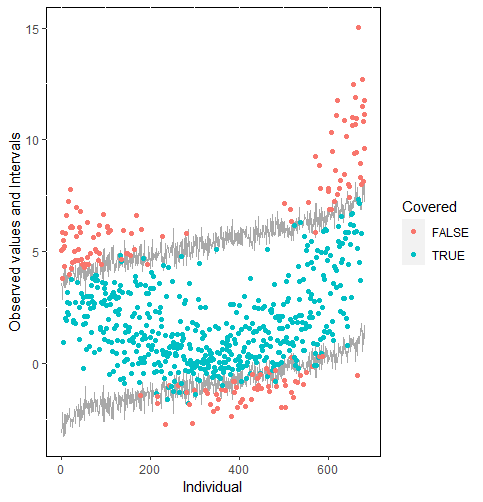
\includegraphics[scale=.5]{plots/plot6.8}
				}
			}
		\end{center}
		\caption{Distribution plots for the first simulation study (quadratic equation with an incomplete outcome) generated under 30\% missing cases and MARr missingness mechanism. The confidence interval is 75\% nominal.}
		\label{fig6_4}
	\end{figure}
	
		\begin{sidewaysfigure}
		\begin{center}
			\resizebox{\textwidth}{!}{
				\subfigure[PC]{
					\label{boxplot:a}
					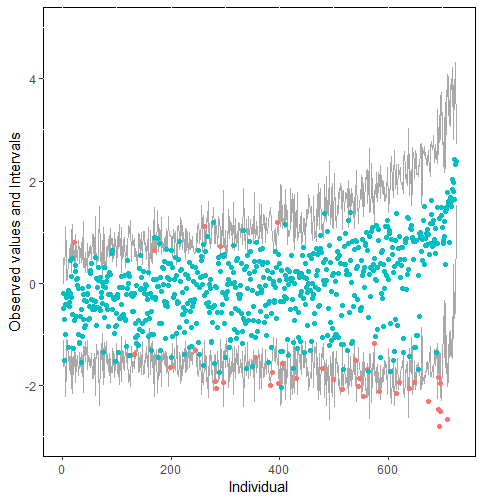
\includegraphics[scale=.5]{plots/plot6.9}
				}
				\subfigure[SMC-FCS]{
					\label{boxplot:b}
					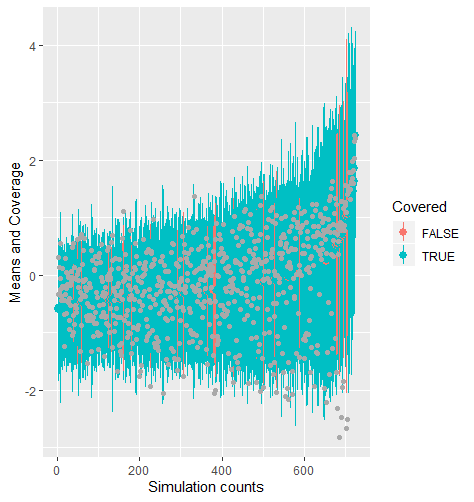
\includegraphics[scale=.5]{plots/plot6.10}
				}
				\subfigure[PMM]{
					\label{boxplot:b}
					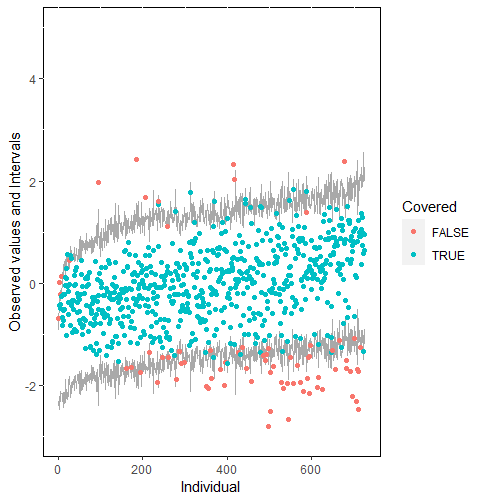
\includegraphics[scale=.5]{plots/plot6.11}
				}
			}
		\end{center}
		\caption{Distribution plots for the second simulation study (quadratic equation with incomplete covariates) generated under 30\% missing cases and MARr missingness mechanism. The nominal level is 95\%.}
		\label{fig6_5}
			\end{sidewaysfigure}
		
			\begin{sidewaysfigure}[ht!]
			\begin{center}
				\resizebox{\textwidth}{!}{
					\subfigure[PC]{
						\label{boxplot:a}
						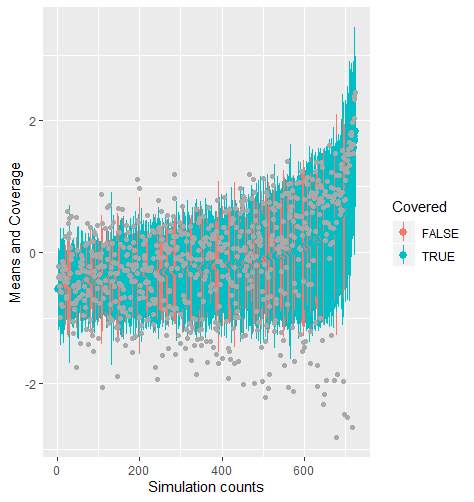
\includegraphics[scale=.5]{plots/plot6.12}
					}
					\subfigure[SMC-FCS]{
						\label{boxplot:b}
						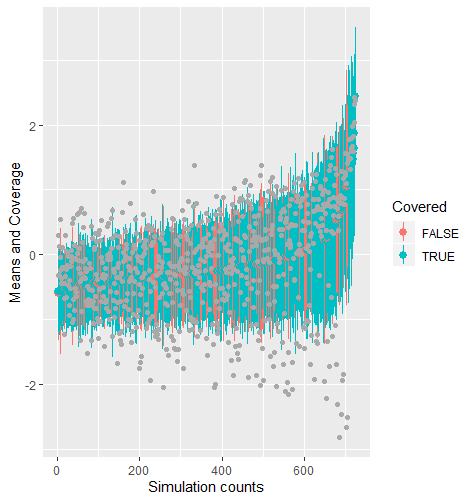
\includegraphics[scale=.5]{plots/plot6.13}
					}
					\subfigure[PMM]{
						\label{boxplot:b}
						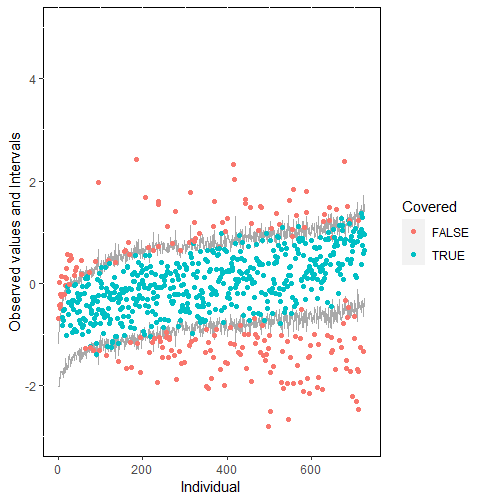
\includegraphics[scale=.5]{plots/plot6.14}
					}
				}
			\end{center}
			\caption{Distribution plots for the second simulation study (quadratic equation with incomplete covariates) generated under 30\% missing cases and MARr missingness mechanism. The nominal level is 75\%.}
			\label{fig6_6}
	
	\end{sidewaysfigure}
	
	\begin{sidewaysfigure}[ht!]
		\begin{center}
			\resizebox{\textwidth}{!}{
				\subfigure[PC]{
					\label{boxplot:a}
					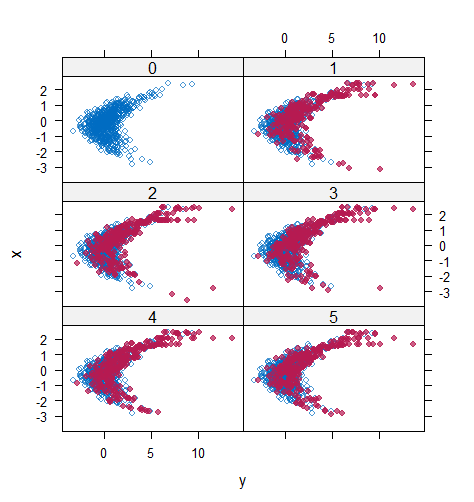
\includegraphics[scale=.5]{plots/plot6.15}
				}
				\subfigure[SMC-FCS]{
					\label{boxplot:b}
					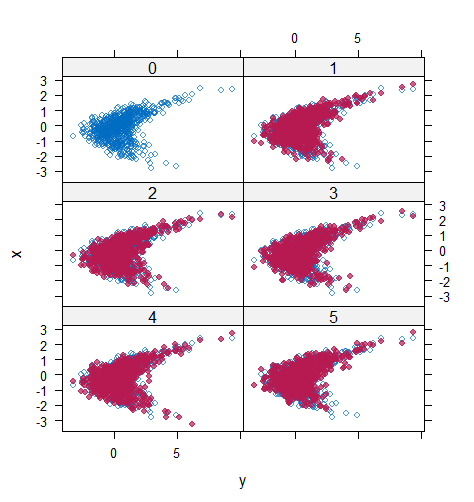
\includegraphics[scale=.5]{plots/plot6.16}
				}
				\subfigure[PMM]{
					\label{boxplot:b}
					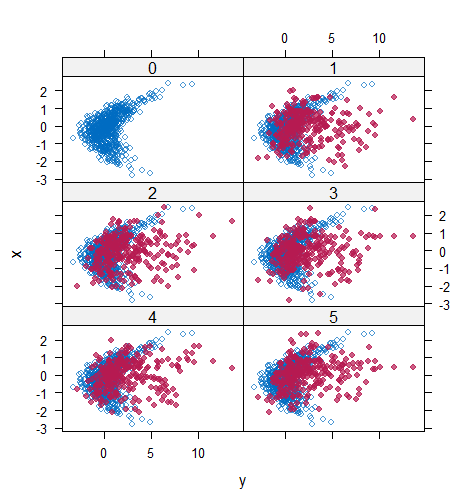
\includegraphics[scale=.5]{plots/plot6.17}
				}
			}
		\end{center}
		\caption{Scatterplots for the second simulation study (quadratic equation with incomplete covariates) generated under 30\% missing cases and MARr missingness mechanism.}
		\label{fig6_7}
	\end{sidewaysfigure}

	\begin{figure}[ht!]
		\begin{center}
			\resizebox{\textwidth}{!}{
				\subfigure[logistic model based on $X$ and $Z$]{
					\label{boxplot:a}
					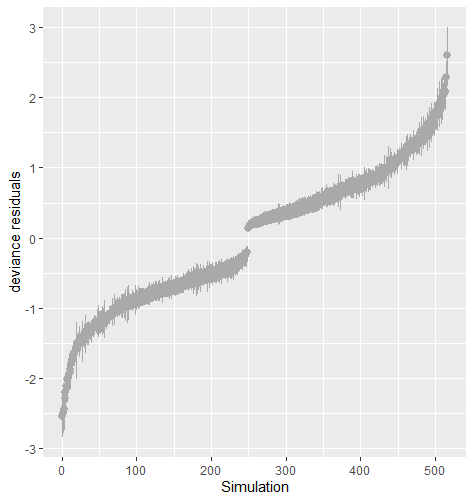
\includegraphics[scale=.5]{plots/plot6.18}
				}
				\subfigure[logistic model based on $Z$]{
					\label{boxplot:b}
					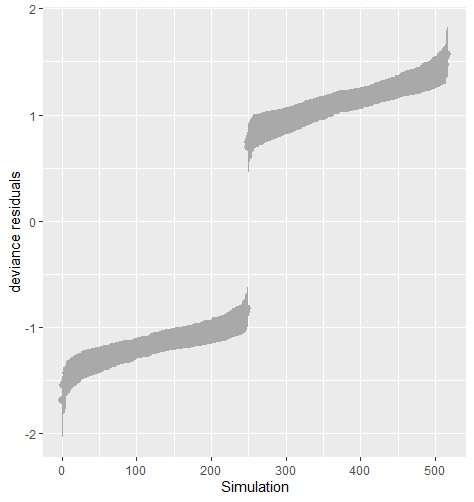
\includegraphics[scale=.5]{plots/plot6.19}
				}
			}
		\end{center}
		\caption{The plot of deviance residuals for the third simulation study (generalized linear model for discrete variables) generated under two logistic regression imputation models. The percentage of missing is 30\%, and the missingness mechanism is MARr.}
		\label{fig6_8}
	\end{figure}
	
	
	
	\begin{figure} [ht!]
		\centering
		\begin{tabular}{cccc}
			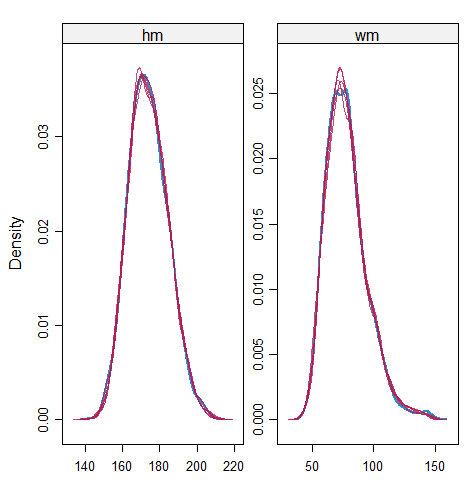
\includegraphics[width=0.3\textwidth]{plots/densitycase1} &
			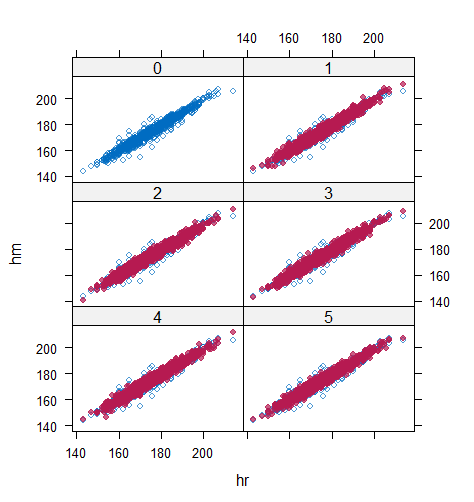
\includegraphics[width=0.3\textwidth]{plots/scattercase1hm} &
			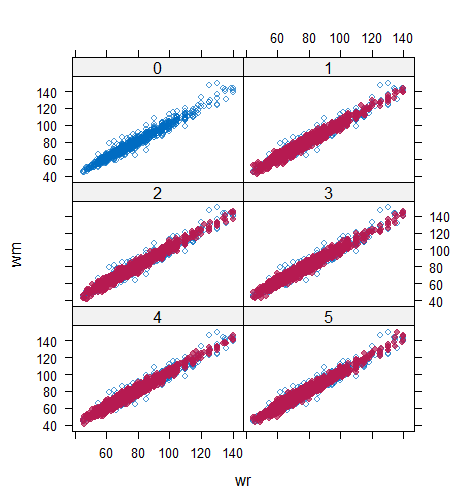
\includegraphics[width=0.3\textwidth]{plots/scattercase1wm} \\
			\textnormal{(a)}  & \textnormal{(b)} & \textnormal{(c)}  \\[6pt]
		\end{tabular}
		\begin{tabular}{cccc}
			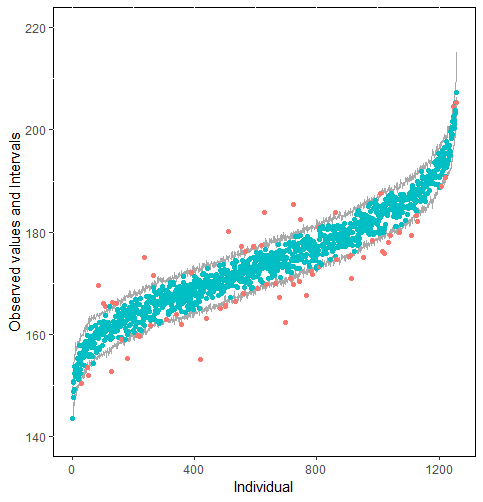
\includegraphics[width=0.3\textwidth]{plots/distributioncase1hm} &
			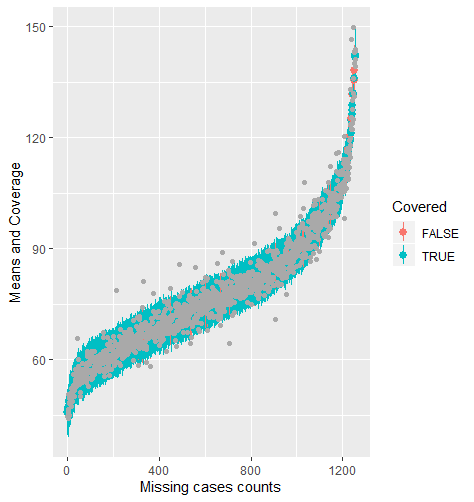
\includegraphics[width=0.3\textwidth]{plots/distributioncase1wm} \\
			\textnormal{(d)}  & \textnormal{(e)}  \\[6pt]
		\end{tabular}
		\caption{Graphical analysis of the BMI data with imputation strategy case 1. (a) density plots, (b) scatter plot of \texttt{hm}, (c) scatter plot of \texttt{wm}, (d) distribution plot of \texttt{hm} and (e) distribution plot of \texttt{wm}.}
		\label{fig6_9}
	\end{figure}
	
	
	\begin{figure} [ht!]
		\centering
		\begin{tabular}{cccc}
			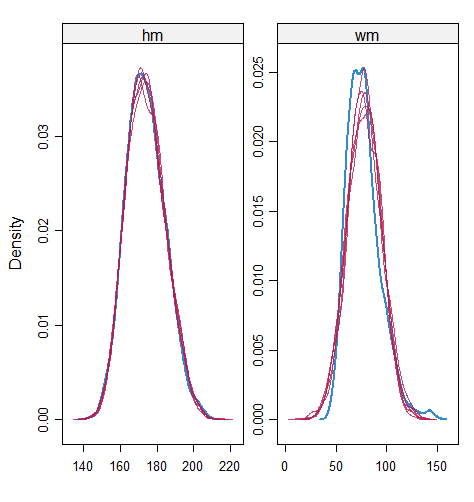
\includegraphics[width=0.3\textwidth]{plots/densitycase2} &
			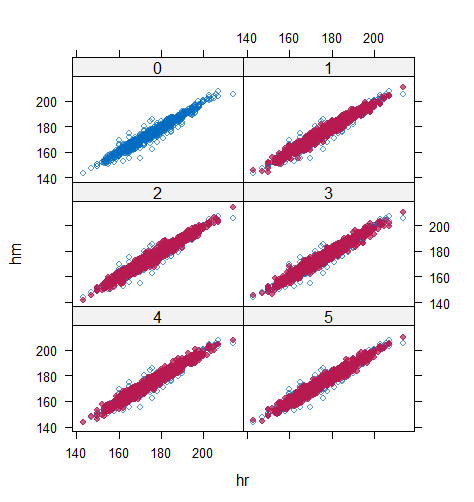
\includegraphics[width=0.3\textwidth]{plots/scattercase2hm} &
			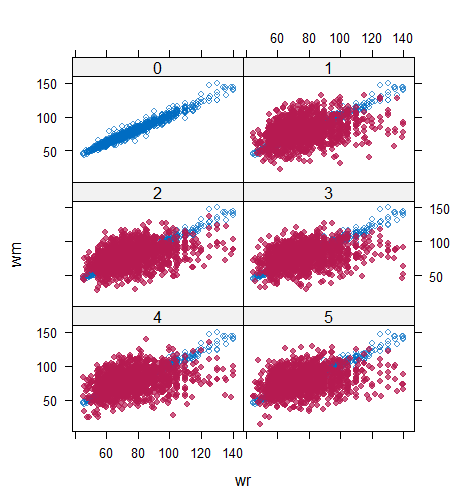
\includegraphics[width=0.3\textwidth]{plots/scattercase2wm} \\
			\textnormal{(a)}  & \textnormal{(b)} & \textnormal{(c)}  \\[6pt]
		\end{tabular}
		\begin{tabular}{cccc}
			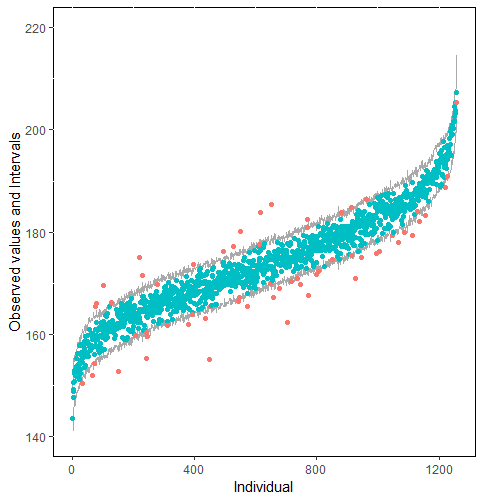
\includegraphics[width=0.3\textwidth]{plots/distributioncase2hm} &
			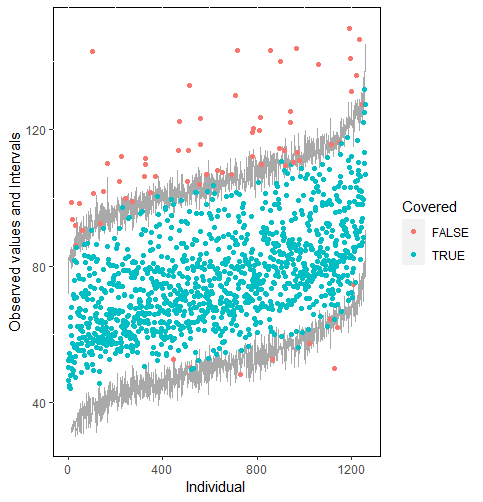
\includegraphics[width=0.3\textwidth]{plots/distributioncase2wm} \\
			\textnormal{(d)}  & \textnormal{(e)}  \\[6pt]
		\end{tabular}
		\caption{Graphical analysis of the BMI data with imputation strategy case 2. (a) density plots, (b) scatter plot of \texttt{hm}, (c) scatter plot of \texttt{wm}, (d) distribution plot of \texttt{hm} and (e) distribution plot of \texttt{wm}.}
		\label{fig6_10}
	\end{figure}
	
	\begin{figure} [ht!]
		\centering
		\begin{tabular}{cccc}
			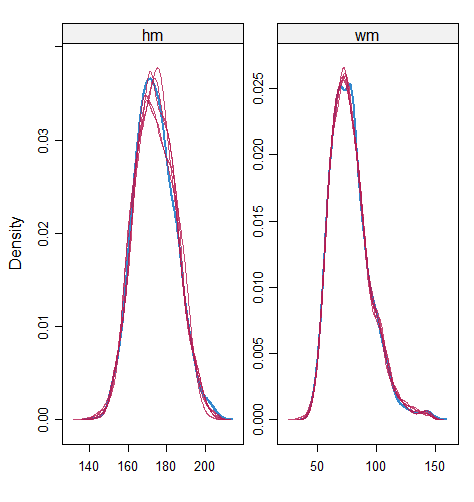
\includegraphics[width=0.3\textwidth]{plots/densitycase3} &
			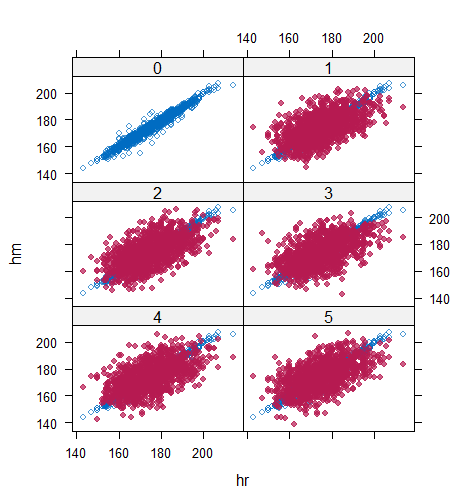
\includegraphics[width=0.3\textwidth]{plots/scattercase3hm} &
			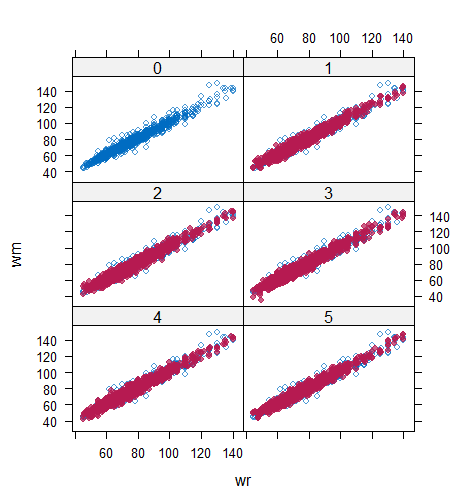
\includegraphics[width=0.3\textwidth]{plots/scattercase3wm} \\
			\textnormal{(a)}  & \textnormal{(b)} & \textnormal{(c)}  \\[6pt]
		\end{tabular}
		\begin{tabular}{cccc}
			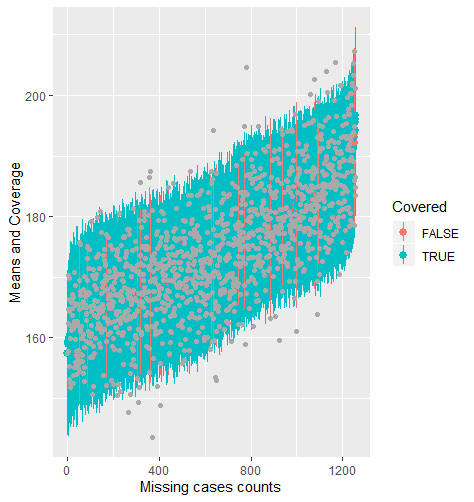
\includegraphics[width=0.3\textwidth]{plots/distributioncase3hm} &
			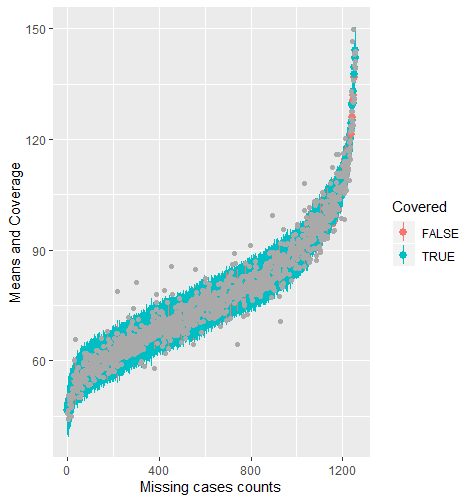
\includegraphics[width=0.3\textwidth]{plots/distributioncase3wm} \\
			\textnormal{(d)}  & \textnormal{(e)}  \\[6pt]
		\end{tabular}
		\caption{Graphical analysis of the BMI data with imputation strategy case 3. (a) density plots, (b) scatter plot of \texttt{hm}, (c) scatter plot of \texttt{wm}, (d) distribution plot of \texttt{hm} and (e) distribution plot of \texttt{wm}.}
		\label{fig6_11}
	\end{figure}
	
	
	\begin{figure} [ht!]
		\centering
		\begin{tabular}{cccc}
			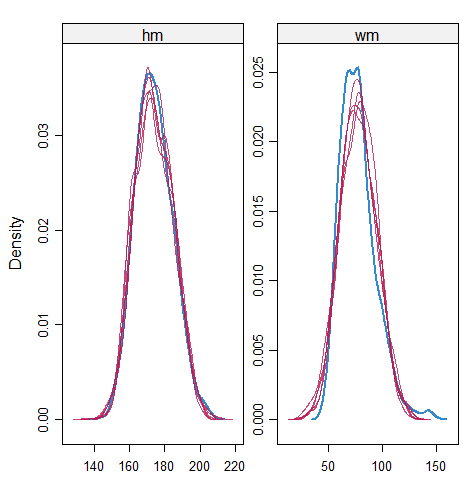
\includegraphics[width=0.3\textwidth]{plots/densitycase4} &
			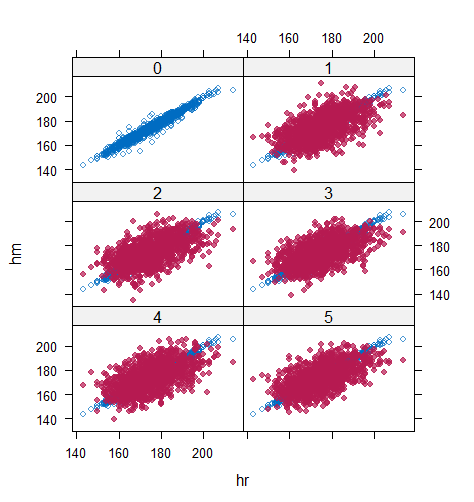
\includegraphics[width=0.3\textwidth]{plots/scattercase4hm} &
			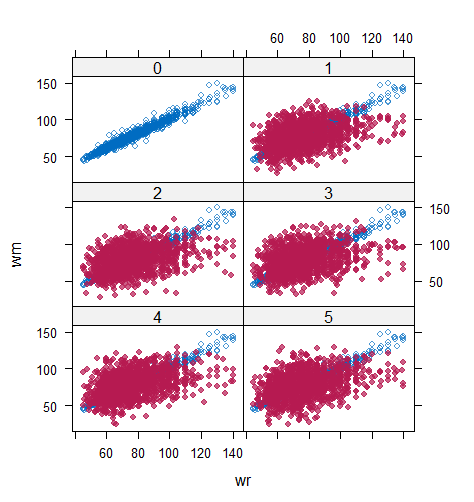
\includegraphics[width=0.3\textwidth]{plots/scattercase4wm} \\
			\textnormal{(a)}  & \textnormal{(b)} & \textnormal{(c)}  \\[6pt]
		\end{tabular}
		\begin{tabular}{cccc}
			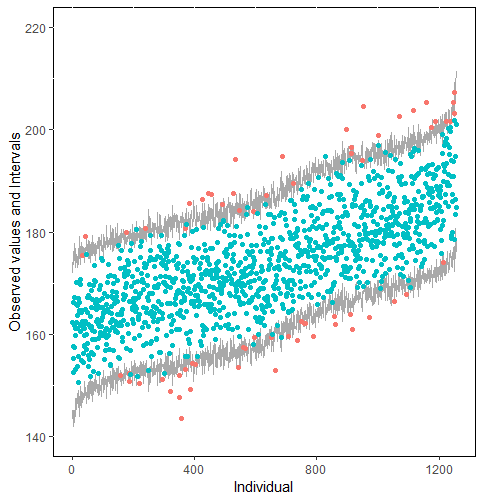
\includegraphics[width=0.3\textwidth]{plots/distributioncase4hm} &
			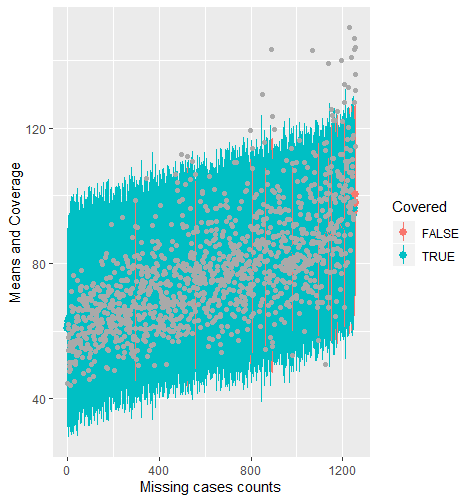
\includegraphics[width=0.3\textwidth]{plots/distributioncase4wm} \\
			\textnormal{(d)}  & \textnormal{(e)}  \\[6pt]
		\end{tabular}
		\caption{Graphical analysis of the BMI data with imputation strategy case 4. (a) density plots, (b) scatter plot of \texttt{hm}, (c) scatter plot of \texttt{wm}, (d) distribution plot of \texttt{hm} and (e) distribution plot of \texttt{wm}.}
		\label{fig6_12}
	\end{figure}
	
	
	
	
